\chapter{Methods}
\label{chapt:methods}

The three models that we implement
in this thesis employ methods
for auditory processing
and trajectory generation
online and in continuous time,
meeting Sermo's criteria
outlined in Section~\ref{sec:sermo}.
Additionally,
we construct spiking neuron models
that implement or interact with those methods
using the Neural Engineering Framework
and Semantic Pointer Architecture.

\section{Auditory periphery models}
\label{sec:periphery-models}

In order to extract a feature vector
from an audio signal
in a biologically plausible manner,
we use models of the auditory periphery
to perform a continuous spectral analysis
of the audio signal.
We compare five existing
auditory periphery model implementations
in the model described in
Section~\ref{sec:ncc}.

\subsection{Gammatone filter}

The Gammatone filter was proposed
in the 1970 (see \cite{johannesma1972,deboer1975,patterson1976}
and has become
the most widely used auditory filter
as it emulates the basic function
of the inner ear,
yet can be implemented efficiently
on general purpose computers.
It capture many of the
psychoacoustical phenomena discussed
in Section~\ref{sec:psychoacoustics},
but does not capture some basic phonemena
(e.g., the auditory filter is symmetric).
However, most importantly,
it can process audio online
and in continuous time,
making it applicable to Sermo.

As described in \cite{patterson1976},
the Gammatone filter has
an impulse response of the form
\begin{equation}
  \text{IR}(t) = t^{n-1} \cos(2 \pi f t) e^{-2 \pi b \text{ERB}(f) t}},
\end{equation}
where $n$ is the order of the filter,
$b$ is a parameter determining the filter bandwidth,
and ERB$(f)$ is the equivalent rectangular bandwidth
of the filter centered at frequency $f$
($\text{ERB}(f) = 24.7 + 0.108f$).
Intuitively, the impulse response
is the convolution of a
carrier signal (the cosine)
and an envelope
(a Gamma function, hence the name Gammatone).
Fourth order Gammatone filters
are the most common
\cite{patterson1992}.
See Figure~\ref{fig:gammatone} for ???.

\fig{gammatone}{0.8}{???}{???}

\cite{slaney1993} proposed an efficient
digital filter implementation
of the Gammatone filter.
The filter is an eighth order
digital filter
implemented as a cascade of four
second order infinite impulse response (IIR) filters
that can be realized
with Direct Form II structure.
The Z-transforms of the
second order filters are
\begin{align*}
  H_1(z) &= \frac{-2 T z^2 + z \left(
            \frac{2 T \cos(2 f \pi T)}{e^{BT}}
            + \frac{2 \sqrt{3 + 2^{1.5}} T \sin(2 f \pi T)}{e^{BT}}
           \right)}
           {\frac{-2}{e^{2BT}} - 2 z^2
           + \frac{4 z \cos(2 f \pi T)}{e^{BT}}} \\
  H_2(z) &= \frac{-2 T z^2 + z \left(
            \frac{2 T \cos(2 f \pi T)}{e^{BT}}
            - \frac{2 \sqrt{3 + 2^{1.5}} T \sin(2 f \pi T)}{e^{BT}}
           \right)}
           {\frac{-2}{e^{2BT}} - 2 z^2
           + \frac{4 z \cos(2 f \pi T)}{e^{BT}}} \\
  H_3(z) &= \frac{-2 T z^2 + z \left(
            \frac{2 T \cos(2 f \pi T)}{e^{BT}}
            + \frac{2 \sqrt{3 - 2^{1.5}} T \sin(2 f \pi T)}{e^{BT}}
           \right)}
           {\frac{-2}{e^{2BT}} - 2 z^2
           + \frac{4 z \cos(2 f \pi T)}{e^{BT}}} \\
  H_4(z) &= \frac{-2 T z^2 + z \left(
            \frac{2 T \cos(2 f \pi T)}{e^{BT}}
            - \frac{2 \sqrt{3 - 2^{1.5}} T \sin(2 f \pi T)}{e^{BT}}
           \right)}
           {\frac{-2}{e^{2BT}} - 2 z^2
           + \frac{4 z \cos(2 f \pi T)}{e^{BT}}},
\end{align*}
where $T$ is is the sampling interval,
$f$ is the characteristic frequency of the filter,
and $B$ controls the bandwidth of the filter
($B = 2 \pi b \text{ERB}(f)$).
See \cite{slaney1993} for the derivation
of the Z-transforms.

\subsection{Log Gammachirp filter}

A primary weakness of the Gammatone filter
is that it responds symmetrically
to power in frequencies above and below
the characteristic frequency of the filter.
In empirically determined auditory filters,
portions of the basilar membrane
are more sensitive to frequencies
below the characteristic frequency,
and have a sharp dropoff in sensitivity
for power in frequencies
above the characteristic frequency.
The family of Gammachirp filters
are IIR filters that remain
computationally efficient,
like the Gammatone filter,
but have an asymmetric frequency response.
They are based on spectral masking experiments
(see Section~\ref{sec:psychoacoustics})
in which the listener has to
detect a brief sinusoidal signal
along ``notched'' white noise,
in which the power spectrum of the noise
at frequencies just above and just below
the frequency of the sinusoid
are set to zero \cite{patterson1976}.
The Log Gammachirp filter,
proposed by \cite{unoki2001}
is an improvement over
the original Gammachirp filter
\cite{irion1997}
in that it is more numerically stable.

The impulse response
of the Log Gammachirp filter is
\begin{equation}
  \text{IR}(t) = t^3 \cos(2 \pi (f t + c \ln(t)) e^{-2 \pi b \text{ERB}(f) t}},
\end{equation}
where $c$ is a ``chirp'' parameter
that affects the asymmetry
of the auditory filter;
typically, $c$ is set to a negative value,
raising the response to lower frequency sounds
and attenuating the response to higher frequency sounds.
See Figure~\ref{fig:log-gammachirp} for a plot of the impulse response.
Unlike the Gammatone impulse response,
the Gammachirp ???more,
use the word frequency sweep

\fig{log-gammachirp}{0.8}{???}{???}

Gammachirp filters are closely related
to Gammatone filters.
In fact, the amplitude spectrum of the Gammachirp is
\begin{equation}
  |G_C(f)| = a_0 \cdot |G_T(f)| \cdot |H_A(f)|,
\end{equation}
where $a_0$ is a scaling factor,
$|G_T(f)|$ is the amplitude sepctrum
of the Gammatone filter,
and $|H_A(f)|$ is the asymmetric function
that depends on the parameter $c$.
See Figure~\ref{???} for a visualization.
The final IIR filter
is designed by determining
an asymmetric filter $H_C(f)$
that simulated the
asymmetric function $H_A(f)$
(see \cite{unoki2001} for details).
The Log Gammachirp improves upon
the original Gammachirp filter
by identifying parameter values
that yield discrepancies
between $H_A(f)$ and $H_C(f)$,
and present an alternative $H_C(f)$
with a parameter that is optimized
to minimize the error between
$H_C(f)$ and $H_A(f)$.

\subsection{Dual resonance nonlinear filter}

The filters discussed to this point
are independent linear filters.
However, as discussed in
Section~\ref{sec:recog-neurobio},
there are many nonlinearities
in the human auditory system,
including at the level of the auditory periphery.

The Dual Resonance Nonlinear (DRNL) filter,
proposed in \cite{lopez2001}
based on earlier work by \cite{meddis2001},
consists of two parallel pathways
that are summed together
(see Figure~\ref{fig:drnl-structure}).
The linear path (top, Figure~\ref{fig:drnl-structure})
scales the input by some gain $g$,
filters the signal through
two or three first-order Gammatone filters,
and then through a cascade of
four second-order low-pass filters.
The non-linear path (bottom, Figure~\ref{fig:drnl-structure})
filters the signal through
three first-order Gammatone filters,
a nonlinear gain,
and three more first-order Gammatone filters.
The filters in the nonlinear path
have the same frequency,
which is the desired characteristic frequency
of the filter,
while the filters in the linear path
have parameters fit to human data.
The result of the linear and nonlinear paths
are summed to yield
the final result of the filter,
which models the velocity of
basilar membrane deflection.

% \fig{drnl-structure}{0.7}{???}{???}
% fig 3 of lopez-poveda

The nonlinear gain in the nonlinear path
is a ``broken stick'' nonlinearity;
i.e.,
\begin{equation}
  y(t) = \text{sign}(x(t)) \min(a |x(t)|, b |x(t)|^c),
\end{equation}
where $x(t)$ is the input signal,
$y(t)$ is the output signal,
and $a$, $b$ and $c$ are parameters.
Like the parameters of the linear path's filters,
these parameters are fit to human data.
Detail on the fitting procedure
and the digital filter implementation
of the filter can be found in \cite{lopez2001}

\fig{drnl}{0.8}{???}{???}

Due to its complexity,
the DRNL impulse response does not have a simple closed form.
However, its impulse response
and frequency response can be simulated;
see Figure~\ref{fig:drnl}?.

\subsection{Dynamic compressive Gammachirp model}

Just as the DRNL filter can be thought of
as an nonlinear extension of Gammatone filters,
the Dynamic Compressive Gammachirp model (DCGC)
\cite{irino2006}
is a nonlinear extension of Gammachirp filters.
It also consists of two pathways,
which, unlike the DRNL,
interact nonlinearly.

% \fig{dcgc-structure}{0.7}{???}{???
% fig 3 from paper

Figure~\ref{fig:dcgc-structure}
gives the overall structure of the filter.
In the control pathway,
the signal is filtered by
a bank of passive Gammachirp filters,
and then a highpass filter.
The signal pathway
also begins with a bank of Gammachirp filters,
and then a highpass filter,
but the high pass filters in the signal pathway
have variable cutoff frequencies
depending on the output of the control pathway.

The filter simulates
several psychoacoustical effects
from masking experiments,
and can be inverted in order to
synthesize audio
from transformed versions
of filter output
\cite{irino2006}.
Like the DRNL filter, it is too complicated
to express the impulse response
in a simple closed form,
but simulated impulse and frequency response
curves are shown in Figure~\ref{fig:dcgc}.

\fig{dcgc}{0.8}{???}{???}

\subsection{Full auditory periphery modeling}

The filters described up to this point
emulate the deflection
of the basilar membrane,
given some audio signal.
These filters are an important part
of a full auditory periphery model,
which should also include
a filter emulating the function
of the outer and middle ear,
a method for transducing
the basilar membrane deflections
into inner hair cell activity,
and a method for generating
action potentials from the inner hair cell activity,
mimicking the function of spiral ganglion cells.
See Figure~\ref{fig:periphmodel} for the full pipeline
of an auditory periphery model.

% ??? figure: hierarchy from wilson et al
% \fig{periphmodel}{0.6}{???}{??? \cite{wilson2005}}

The middle ear function...
??? figure out

For transducing the inner hair cell activity,
we rectify and compress the output
of the auditory filter model
to account for two effects.
First, the basilar membrane may deflect
positively or negatively
(as can be seen in the impulse response
in Figure~\ref{fig:gammatone}),
but only positive deflections result in
inner hair cell activity.
Second, the amount of inner hair cell activity
does not linearly increase with
membrane deflection;
the activity is ``compressed''
as the deflection increases.
These effects are modeled by
\begin{equation} \label{filter-compress}
  f(x) =
  \begin{cases}
    x^{1 / 3} &\text{if } x \ge 0 \\
    0 &\text{if } x < 0.
  \end{cases}
\end{equation}
The result of equation~\eqref{filter-compress}
is interpreted as the inner hair cell activity,
which is the input to a simulated neuron.
Synapses and neurons are simulated with Nengo;
see Section~\ref{sec:nengo} for details.

\subsection{Tan \& Carney model}

Finally, we also test
an auditory periphery model
presented in \cite{tan2003}
which takes into account
the full auditory periphery pathway
in Figure~\ref{fig:periphmodel}.

\fig{tancarney-structure}{0.8}{???}{???}

The model, depicted in
Figure~\ref{fig:tancarney-structure},
consists of a middle ear model,
a auditory filter consisting
of a control path and signal path,
and an inner hair cell
and synapse model.
The output of the model
is the instantaneous firing rate
of spiral ganglion cells
connected to inner hair cells
sensitive to a particular
characteristic frequency.

The signal path in the model
consists of a linear bandpass filter
with two eight-order poles
and one fourth-order pole,
their complex conjugates,
and a tenth-order zero
on the real axis.
Despite this complexity,
\citeauthor{tan2003}
state that these poles and zero
are the minimum number required
to capture physiological effects
like frequency glides
and sharp frequency response curves.

% \fig{tancarney}{0.8}{???}{???}
% ??? fig impulse, freq

The bandwidth and gain of the linear filter
in the signal path is controlled
by the output of the control path,
which can be thought of as
implementing the compression
mentioned in the previous section.
The control path cascade consists of
a nonlinear wideband filter,
a symmetric nonlinear function,
an asymmetric nonlinear Boltzmann function,
and a second-order lowpass filter
with a cutoff frequency of 800 Hz.
As mentioned above,
the output of the control path
controls the bandwidth
of the signal path,
but it also is fed back
into the start of the control path
to control the bandwidth of the initial
wideband filter.

In the full model, the output of the signal path
is used to simulate an inner hair cell,
and the synapse between an inner hair cell
and a spiral ganglion cell
\cite{{zhang2001}.
The IHC model
consists of a log-sigmoid transfer function
and a seventh-order lowpass filter.
The synapse model is a three-store
diffusion model \cite{carney1993},
which generates the instantaneous
rate of a spiral ganglion cell.
However, in this thesis,
we will instead use a synapse
and neuron model in Nengo
to reduce computational complexity
and make the five models more consistent.

\subsection{Brian hears software}
\labec{sec:brian-hears}

The \textit{Brian hears} software
\cite{fontaine2011}
provides implementations
of the five models described above.
\textit{Brian hears} is part of the
\textit{Brian} package,
which is a general purpose
neural simulator capable
of simulating spiking neural networks
with relatively high precision
but slow speed
(see \cite{bekolay2013} for benchmark results).
Due in part to its slow speed,
we use \textit{Brian} only for
the auditory periphery model implementations
provided in the \textit{Brain hears} subpackage,
and use Nengo (described below)
for all other model implementations.

\section{Dynamic movement primitives}
\label{sec:methods-dmp}

Dynamic movement primitives (DMPs)
are a method for planning and controlling trajectories
that requires little parameter tuning
and is stable for trajectories
with many degrees of freedom.
DMPs were originally proposed
by \cite{schaal2005,schaal2006},
reformulated and refined by \cite{ijspeert2007},
and simplified for use in spiking neural networks
by \cite{dewolf2014}.
Here, we summarize the essential aspects
of the DMP framework as described by \cite{dewolf2014},
but invite interested readers to
the previously cited works
and \cite{vijayakumar2005,ijspeert2013}
for further details and extensions.

DMPs use dynamical systems
with specified, stable behavior
to generate trajectories
with more complicated behavior.
The main insight in the DMP framework
is to define two separate systems,
a point attractor,
and a ``canonical system.''
The point attractor pushes
the system state to
a goal, $g$, with dynamics
\begin{equation}
  \label{dmp-pointattractor}
  \tau\ddot{y} = \alpha_y(\beta_y(g - y) - \dot{y}) + f(x, g),
\end{equation}
where $y$ is the system state,
$\dot{y}$ is the system velocity,
and $\alpha_y$ and $\beta_y$ are gain terms.
$\tau$ is a scaling term
that enables to system to operate
at different timescales,
and also appears in the definition
of the canonical system.

$f(x, g)$ is a function
of the canonical system
called the ``forcing function.''
In the discrete, one-time action case,
the canonical system
has state $x$ that evolves
with dynamics
\begin{equation}
  \label{dmp-discrete}
  \tau\dot{x} =
  \begin{cases}
    1 &\text{if } x < 1 \\
    0 &\text{if } x \ge 1,
  \end{cases}
\end{equation}
Typically the initial value of $x$
is set to 0,
so the discrete forcing function
is defined over the range $[0, 1]$.
In the rhythmic case,
the state evolves with
2D oscillator dynamics
\begin{align}
  \tau \dot{x_1} &= -2 \pi x_2 \nonumber \\
  \tau \dot{x_2} &= 2 \pi x_1.
  \label{dmp-rhythmic}
\end{align}

% \fig{dewolf}{0.5}{???}{???}
% ??? Figure 3.1 from dewolf thesis

The forcing function $f(x, g)$ is
the weighted sum
over some basis functions
$\psi_i$
(see Figure~\ref{fig:dewolf}).
In the discrete case,
the basis functions are evaluated
for the system state $x$ directly.
In the rhythmic case,
the basis functions are evaluated
for $\frac{1}{2\pi}\tan^{-1}\left(\frac{x_2}{x_1}\right) + \frac{1}{2}$,
which maps the 2D oscillator state
to the range $[0, 1]$,
allowing the forcing function to be defined
as a function of $x$ over the range $[0, 1]$
in both cases.
The goal $g$ is used
to scale the system state $x$ depending on
the initial distance to the goal.
The final equation is
\begin{equation}
  \label{dmp-forcing-func}
  f(x, g) = \frac{\sum_{i=1}^N \psi_i w_i}{\sum_{i=1}^N \psi_i} \, x(g - y_0),
\end{equation}
where $w_i$ is the weight associated with
basis function $\psi_i$ and $y_0$
is the initial position of
the system state.

Typically, Gaussian functions
tiling the range of $x$ with some overlap
are used as the basis functions
for the forcing function
(as are used in Figure~\ref{fig:dewolf}).
\cite{dewolf2014} dewolf showed that
the response curves of spiking neurons
could be used as the
basis functions instead
(as is done for general function approximation
in the Neural Engineering Framework;
see Section~\ref{sec:nef}).

\section{Neural Engineering Framework (NEF)}
\label{sec:nef}

The Neural Engineering Framework
(NEF; \cite{eliasmith2004})
provides a unified method of
representing and transforming information
in spiking neural networks
such that they can implement
arbitrary dynamical systems.
The NEF is the most prominently used
tool in this thesis,
and greatly influenced the
development of the conceptual Sermo model
through the constraints and assumption
inherent in the NEF.

The NEF defines three principles that
can be used to build large-scale networks
using any spiking or non-spiking neuron model.

\subsection{Representation}
\label{sec:representation}

The representation scheme in the NEF
is based on \textit{population coding},
which was first proposed by
\cite{georgopoulos1986}
based on experiments in monkey cortex.
Population coding is a type of distributed representation,
theorizing that an ensemble of neurons
collectively represents information.
In the original \cite{georgopoulos1986|} experiment,
the ensemble of neurons coded
for the direction of a reach;
in other words,
a two-dimensional vector.
The NEF generalizes
this type of neural representation to
$n$-dimensional vector spaces,
and higher-level representations
like functions and vector fields.

The representation principle in the NEF
defines a nonlinear encoding process
and a weighted linear decoding process.
In encoding,
we aim to distribute the representation
of a vector, $\V{x}$,
by injecting current, $J$,
in a neuron model,
yielding neural activity $a(J)$.
The exact neural activity depends on
a nonlinear function, $G[\cdot]$,
which is defined by the neuron model.

In this thesis, we will primarily use
leaky integrate-and-fire (LIF) neurons.
LIF neurons are defined by the differential equation
\begin{equation*}
  \frac{dV}{dt} = - \frac{1}{RC} \left(V(t) - J(t) R\right),
\end{equation*}
where $R$ is resistance, $C$ is capacitance,
and $V(t)$ is voltage at time $t$.
When $V(t)$ reaches a threshold $V^{th}$,
the model ``spikes,''
meaning that the time of the spike,
$t_s$, is recorded,
and the voltage, $V(t)$, is reset to baseline.

In the general case,
the neural activity $a(J)$
is determined by direct simulation.
However, the LIF neuron is
simple enough that it can be
solved for directly.
\begin{equation}
  \label{eq:lif-activity-j}
  a(J) = G[J] =
  \begin{cases}
    \textstyle
    \frac{1}{\tau^{ref} - \tau^{RC} \ln \left(1 - \frac{J^{th}}{J}\right)} & \text{if } J > J^{th} \\
    0 & \text{otherwise},
  \end{cases}
\end{equation}
where $\tau^{ref}$ is the refractory time constant,
$\tau^{RC}$ is the RC time constant,
and $J^{th}$ is the current threshold
above which the neuron will spike.

The remaining question, then,
is how to relate the desired vector
$\V{x}$ to the input current
$J$ for each cell.
To do this, we first assign some
attributes to each neuron in the ensemble
that will represent $\V{x}$.
\begin{itemize}
  \item $\V{e}$ is a unit length \textit{encoder}
    that specifies the direction in vector space
    to which the neuron is sensitive.
  \item $alpha$ is a gain term that scales
    incoming signals.
  \item $J^{bias}$ is background current that
    is always present, biasing the cell
    to spike or not spike at varying input levels.
\end{itemize}
Then, the amount of current that is injected
in that neuron is
\begin{equation} \label{eq:encoding}
  J(\V{x}) = \alpha \V{e} \cdot \V{x} + J^{bias},
\end{equation}
where $\cdot$ is the dot product.
Since the dot product gives us
the projection of one vector on another,
it is high when the two vectors are similar;
effectively, the $\V{e} \cdot \V{x}$ term
tells us that neurons fire
more strongly when the input signal
is similar to the part of the vector space
that the neuron is sensitive to.
That similarity is then scaled by $alpha$
and biased by $J^{bias}$,
giving us the input current for each neuron.

The parameters associated with each neuron
can be chosen in several ways.
The most common way is to randomly sample
a distribution that is constrained
by knowledge of the system being modeled.
For example, if we are modeling an ensemble
of Purkinje cells, then the gains should
have the cell spike at between 1--150 Hz
for normal input signals.
If we are are modeling
an ensemble of brightness sensitive cells,
and there are usually
twice as many `on' neurons as `off' neurons,
then we would bias the
random generation of encoders appropriately.
Other times, the neuron parameters
are chosen in order to better implement
a particular function.
For example, if we are attempting to
implement a thresholding function
(e.g., $f(\V{x}) = 1 \text{if } \V{x} > 0.9$)
then using all positive encoders
and biases such that the cells
will only fire when $\V{x} > 0.9$.

In decoding, the goal is to estimate
the originally encoded vector $\V{x}$.
The NEF does this with a weighted sum
of the neural activities with a set
of decoding weights, $\V{d}$.
I.e.,
\begin{equation}
  \label{vec}
  \V{\hat{x}} = \sum_{i=0}^n \V{d}_i a_i,
\end{equation}
where $\V{\hat{x}}$ is the
decoded estimate of the encoded vector $\V{x}$,
$\V{d}_i$ is the decoding weight for neuron $i$,
and $a_i$ is the activity of neuron $i$.

To determine the decoding weights $\V{d}$
we minimize the reconstruction error
$\V{x} - \V{\hat{x}}$
by setting up the relation
\begin{equation*}
  \V{Ad} = \V{X},
\end{equation*}
where $\V{X}$ is a set of sample points
in the vector space,
and $A$ is a matrix with the activities
of all neurons for all neurons;
i.e.,
\begin{equation*} \label{eq:decoding}
  \label{A}
  \V{A} =
  \begin{bmatrix}
    a_0(X_0) & a_1(X_0) & \dots  & a_n(X_0) \\
    a_0(X_1) & a_1(X_1) & \dots  & a_n(X_1) \\
    \vdots & \vdots & \ddots & \vdots \\
    a_0(X_m) & a_1(X_m) & \dots  & a_n(X_m).
  \end{bmatrix}
\end{equation*}
This equation is in the form
of a linear least squares problem,
which can be solved with standard methods
\cite{lawson1974}.
See Figure~\ref{fig:dec-scalar} for an illustration
of how the decoding vectors
result in an estimate of the encoded vector.

% \begin{figure}[ht!]
%   \centering
%   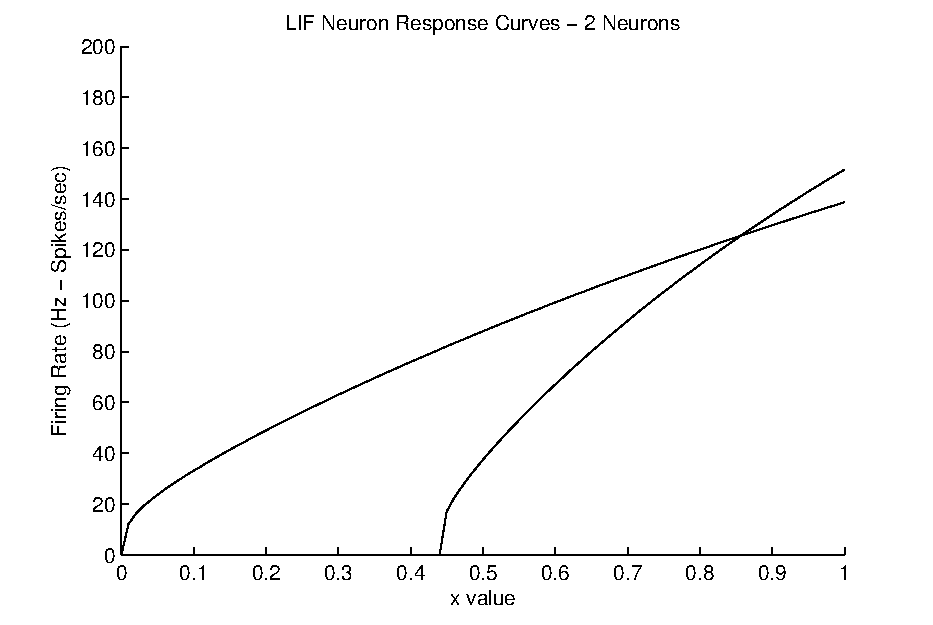
\includegraphics[width=0.45\columnwidth]{lif_est_resp_2}
%   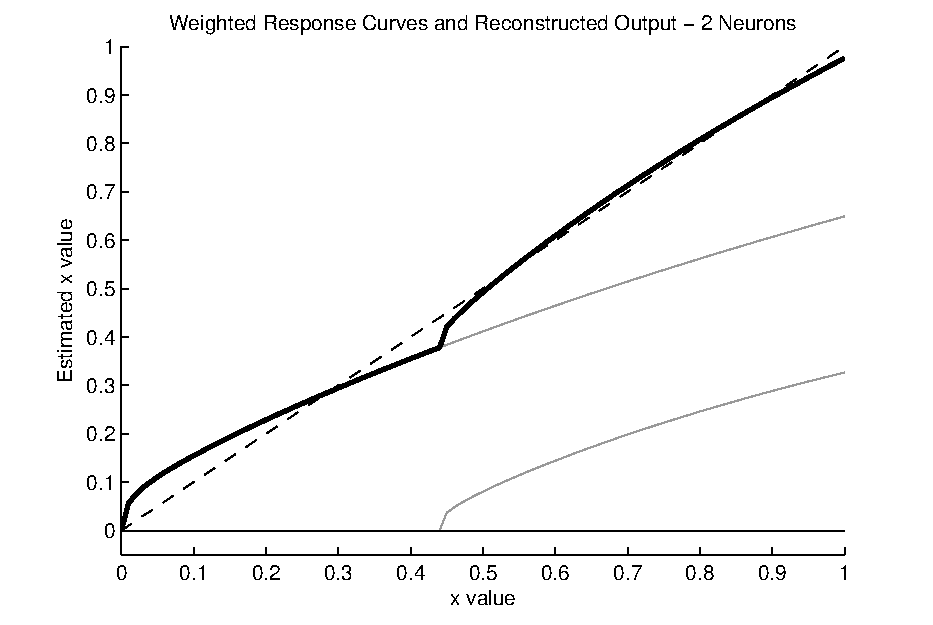
\includegraphics[width=0.45\columnwidth]{lif_est_out_2} \\
%   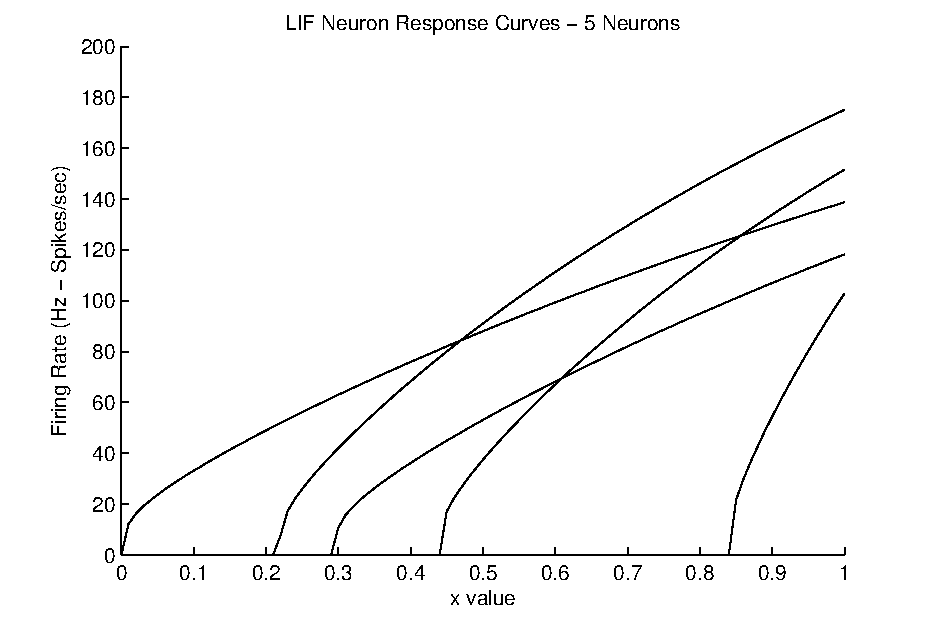
\includegraphics[width=0.45\columnwidth]{lif_est_resp_5}
%   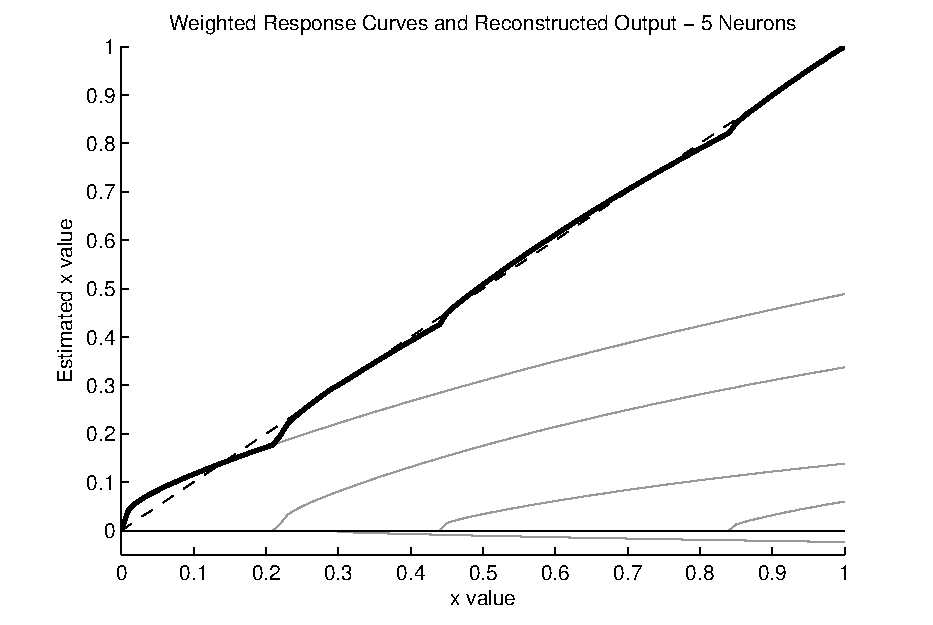
\includegraphics[width=0.45\columnwidth]{lif_est_out_5} \\
%   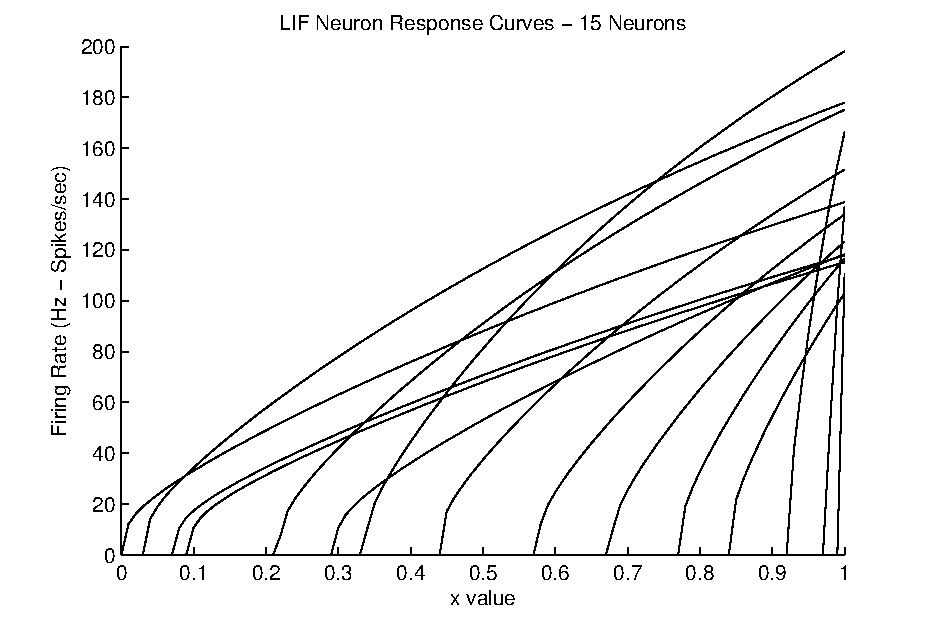
\includegraphics[width=0.45\columnwidth]{lif_est_resp_15}
%   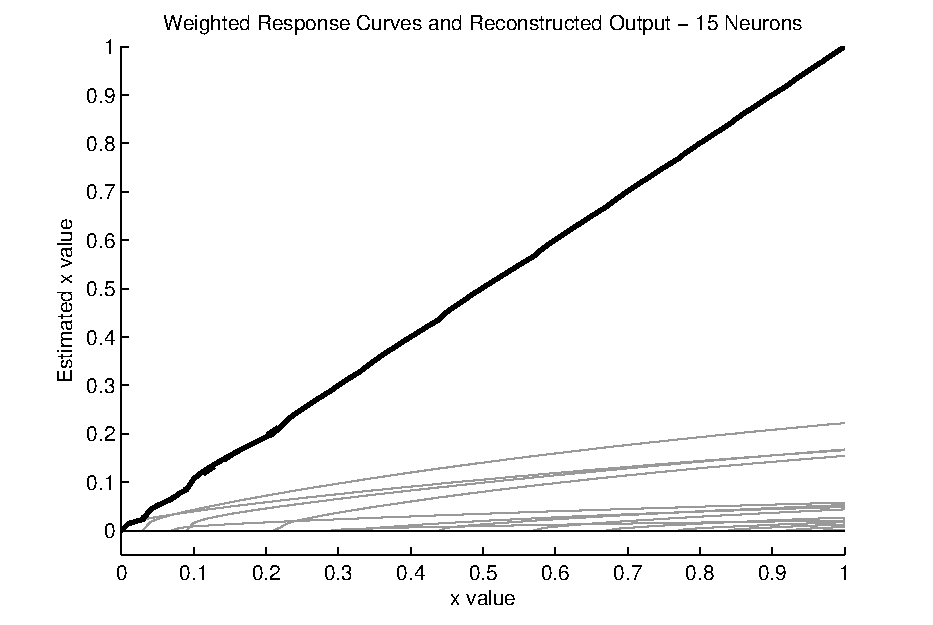
\includegraphics[width=0.45\columnwidth]{lif_est_out_15}
%   \caption{Illustration showing how the tuning curves of a population of LIF
%     neurons can be linearly combined to estimate an input signal, $x$. From
%     \cite{Choo2010}.}
%   \label{fig:dec-scalar}
% \end{figure}

For neurons with instantaneous rate equations,
like the LIF neuron (see Equation~\eqref{eq:lif-activity-j}),
the description to this point
is sufficient to encode and decode information.
However, to deal with spiking neuron models,
we must explicitly consider time,
which to this point has been an implicit
part of all of the equations.
We model neural spikes as
Dirac $\delta$ functions,
and define the time-varying
neural activity as
\begin{equation}
  \label{a(t)}
  a(t) = \sum_s \delta(t - t_s) * h(t) = \sum_s h(t - t_s),
\end{equation}
where $s$ is the set of spike times,
$*$ is the convolution operator,
and $h(\cdot)$ is a filter designed to
model the change in a neuron's current
as a result of an incoming spike
of neurotransmitter.\footnote{
  Equation~\eqref{a(t)} is also how we determine
  the steady state activity of each neuron in
  equation~\eqref{A} for neuron models
  that do not have an analytical
  instantaneous rate equation.}
Typically, we emulate post-synaptic current curves
recorded empirically by using a decaying exponential;
i.e.,
\begin{equation}
  h(t) = e^{-t / \tau^{PSC}},
\end{equation}
where $\tau^{PSC}$ is the time constant
of the exponential curve decay,
designed to match
a recorded post synaptic current (PSC) curve.

Putting these equations together,
we get the final expression for
the decoded estimate of the input $\V{x}$
using spiking neuron models,
\begin{equation}
  \label{dec-time}
  \V{\hat{x}}(t) = \sum_{i=0}^n \V{d}_i \sum_{s_i} h(t-t_{s_i}).
\end{equation}
See Figure~\ref{fig:temporal-dec} for an illustration of
the decoding process.

% \scalefigonesumm{temporal-dec}{0.8}{Decoding a time-varying
%   scalar signal using a filtered spike train.}
%   {Example of decoding a time-varying
%   scalar signal using a filtered spike train. For each spike, the
%   filter $h(t)$ is pasted in, weighted by the decoding weight
%   (1 or -1 in this case). Recreated from \cite{Eliasmith2011}.}

\subsection{Transformation}

In the representation principle,
we treated neurons as though
it were possible to directly inject current in them.
While direct current injections
can make sense for modeling
sensory systems,
the majority of neurons
receive their input from other neurons.
In the transformation principle,
the NEF defines an alternately weighted
linear decoding
that can transmit functions
of the vector represented
by one ensemble to another ensemble
through a connection weight matrix.

Given some neuron $j$
in an ensemble downstream
of an ensemble with neurons indexed by $i$,
the input current to neuron $j$ is
\begin{equation}
  \label{Jin}
  J_j = \sum_{i=0}^n \omega_{ij} a_i + J_j^{bias},
\end{equation}
where $omega_{ij}$ is the strength of the connection
between neurons $i$ and $j$.

Consider the case in which we want
an ensemble to represent
the same vector as the ensemble
providing it input;
i.e., we want to implement the function
$\V{y} = f(\V{x}) = \V{x}$.
Equation~\eqref{...} tells us how
we can approximate $\V{x}$, so let us
substitute that approximation
into equation~\eqref{...}.
\begin{align} \label{eq:jin-xhat}
  J_j &= \alpha_j \V{e}_j \cdot \V{\hat{x}} + J_j^{bias} \nonumber \\
      &= \alpha_j \V{e}_j \cdot \sum_{i=0}^n \V{d}_i a_i + J_j^{bias} \nonumber \\
      &= \sum_{i=0}^n \alpha_j \V{e}_j \cdot \V{d}_i a_i + J_j^{bias}
\end{align}

Setting \eqref{...} equal to \eqref{...},
we can rearrange terms to
obtain an equation for $\omega_{ij}$.
\begin{align} \label{eq:omega}
  \sum_{i=0}^n \omega_{ij} a_i + J_j^{bias} &= \sum_{i=0}^n \alpha_j \V{e}_j \cdot \V{d}_i a_i + J_j^{bias} \nonumber \\
  \omega_{ij} &= \alpha_j \V{e}_j \cdot \V{d}_i
\end{align}

Since the decoding process is linear,
we can implement any linear function
by introducing a matrix $L_{ji}$
that performs a different combination
of the downstream ensemble's encoders, $\V{e_j}$,
and the upstream ensemble's decoders, $\V{d_i}$.
\begin{equation} \label{eq:linear-trans}
  \omega_{ij} &= \alpha_j \V{e}_j \V{C}_{ji} \V{d}_i
\end{equation}

Since the decoding process is
a weighted summation,
we can compute the sum of
vectors of the same length
by representing those vectors
with separate ensembles
and making a connection
from each ensemble to the downstream ensemble.
\begin{align}
  \label{eq:nef-sum}
  J_j &= J_j^{\V{x}} + J_j^{\V{y}} + J_j^{bias} \nonumber \\
      &= \sum_i \omega_{ij}^{\V{x}}a_i^{\V{x}} + \sum_i \omega_{ij}^{\V{y}}a_i^{\V{y}} + J_j^{bias} \nonumber \\
  \omega_{ij}^{\V{x}} &= \alpha_j \V{e}_j \V{C}^{\V{x}}_{ji} \V{d}_i^{\V{x}} \text{ and }
  \omega_{ij}^{\V{y}} = \alpha_j \V{e}_j \V{C}^{\V{y}}_{ji} \V{d}_i^{\V{y}},
\end{align}
and so on for any number of input ensembles.

Nonlinear transformations
of some vector $\V{x}$ can be implemented
by computing a new set of decoding weights,
$\V{d}^{f(\V{x})$,
which minimizes the reconstruction error
between the estimate $\V{\hat{x}}$
and the result of applying the function,
$f(\V{x})$. I.e., equations~\eqref{...} and \eqref{...} become
\begin{align*}
  \V{A}^{f(\V{x})}d^{f(\V{x})} &= f(\V{X}) \\
  \V{A}^{f(\V{x})} &=
  \begin{bmatrix}
    a_0(f(X_0)) & a_1(f(X_0)) & \dots  & a_n(f(X_0)) \\
    a_0(f(X_1)) & a_1(f(X_1)) & \dots  & a_n(f(X_1)) \\
    \vdots & \vdots & \ddots & \vdots \\
    a_0(f(X_m)) & a_1(f(X_m)) & \dots  & a_n(f(X_m)),
  \end{bmatrix}
\end{align*}
and the remaining equations only change
in the set of decoding weights used.
See Figure~\ref{fig:dec-func} for an illustration
of decoding a nonlinear function.

% \begin{figure}[ht!]
%   \centering
%   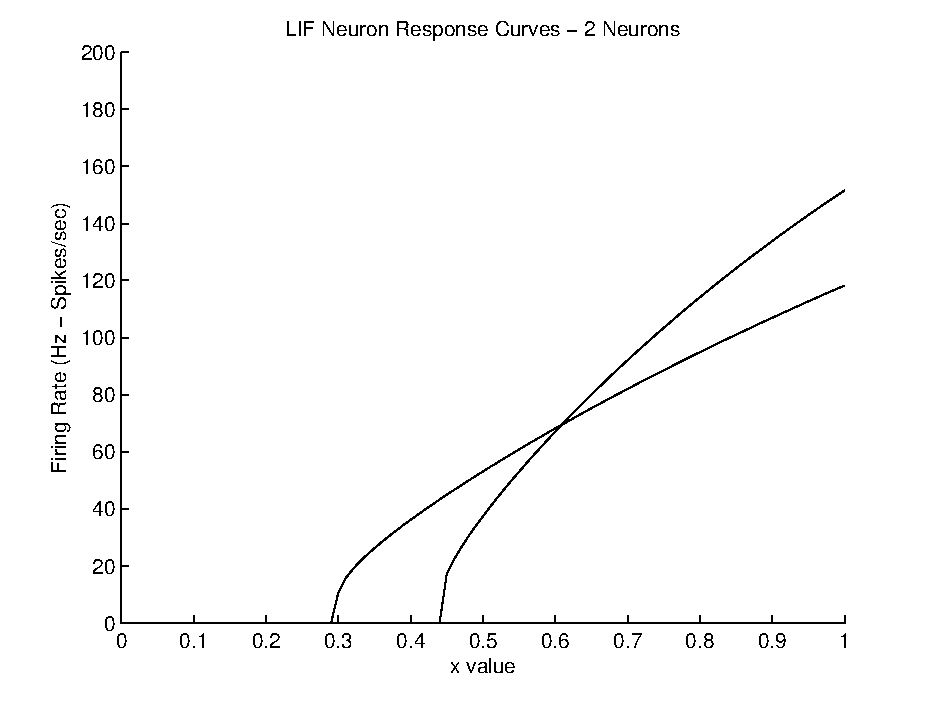
\includegraphics[width=0.45\columnwidth]{lif_func_resp_2}
%   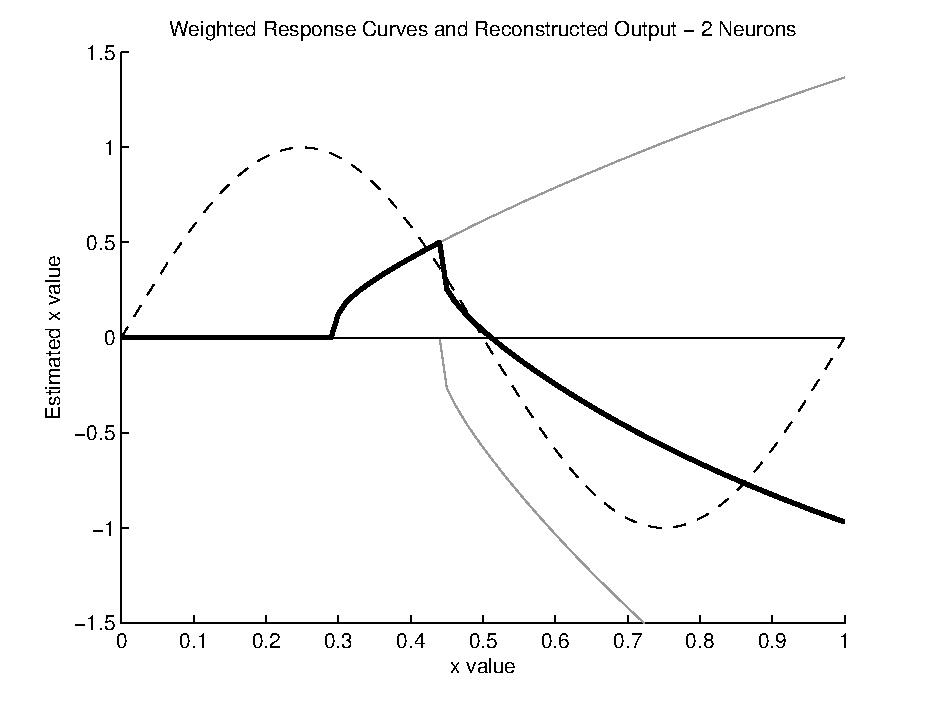
\includegraphics[width=0.45\columnwidth]{lif_func_out_2} \\
%   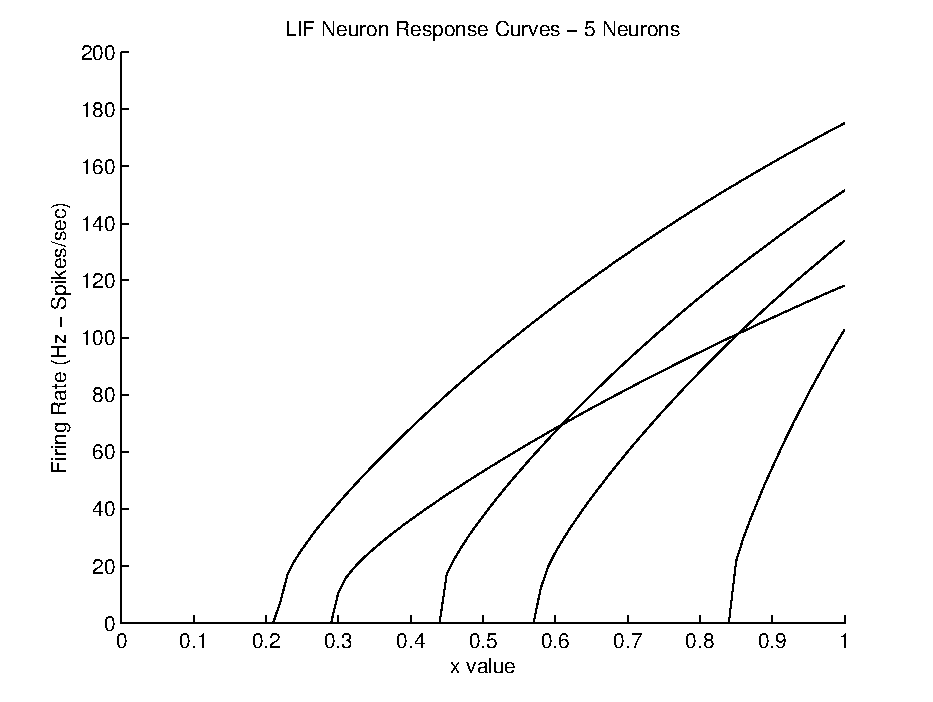
\includegraphics[width=0.45\columnwidth]{lif_func_resp_5}
%   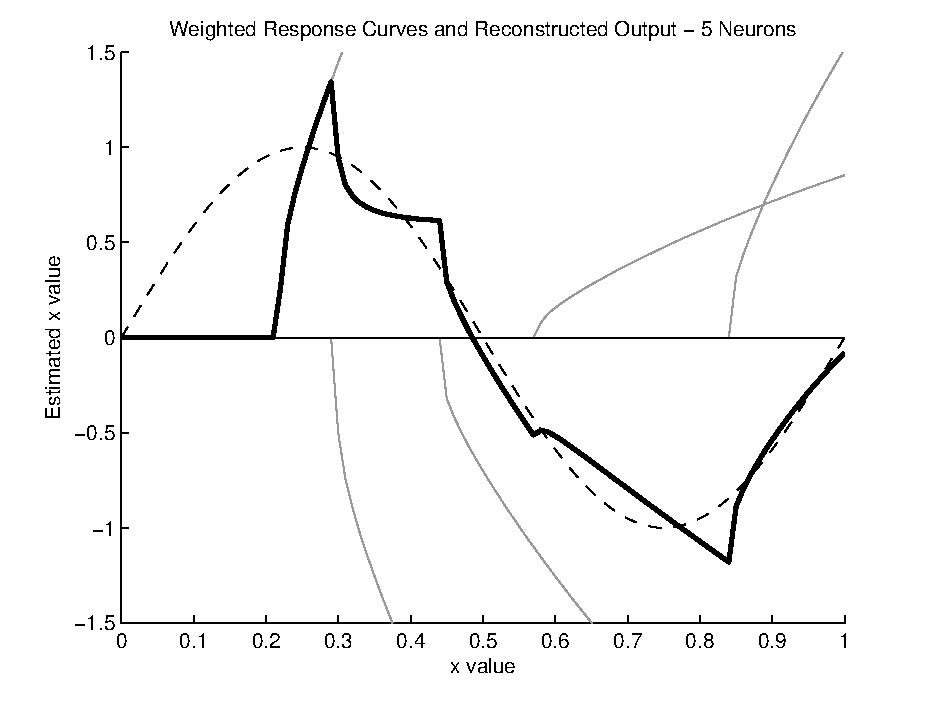
\includegraphics[width=0.45\columnwidth]{lif_func_out_5} \\
%   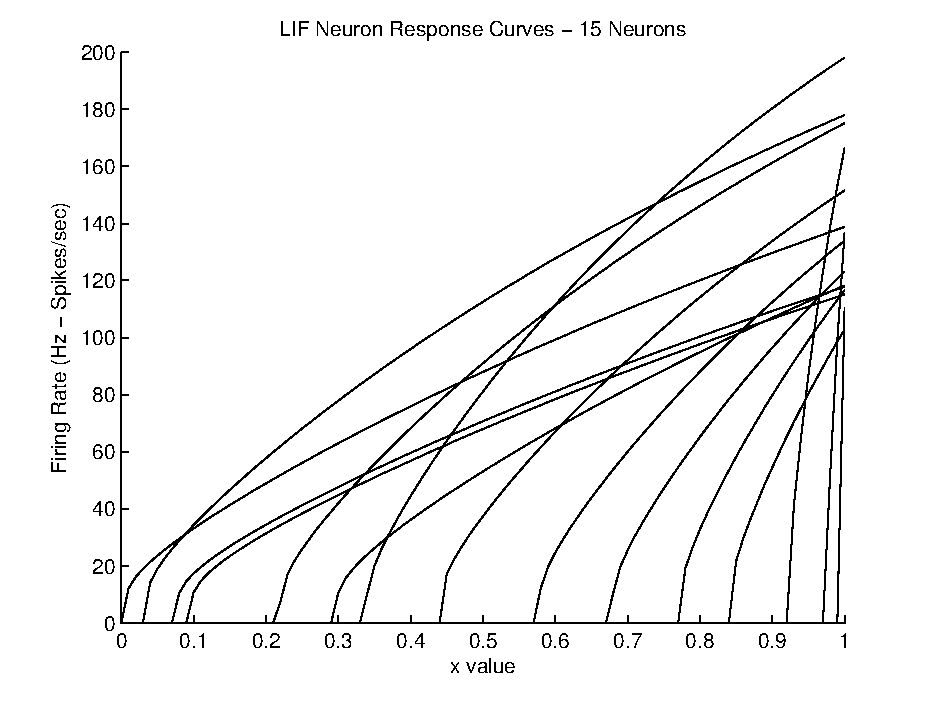
\includegraphics[width=0.45\columnwidth]{lif_func_resp_15}
%   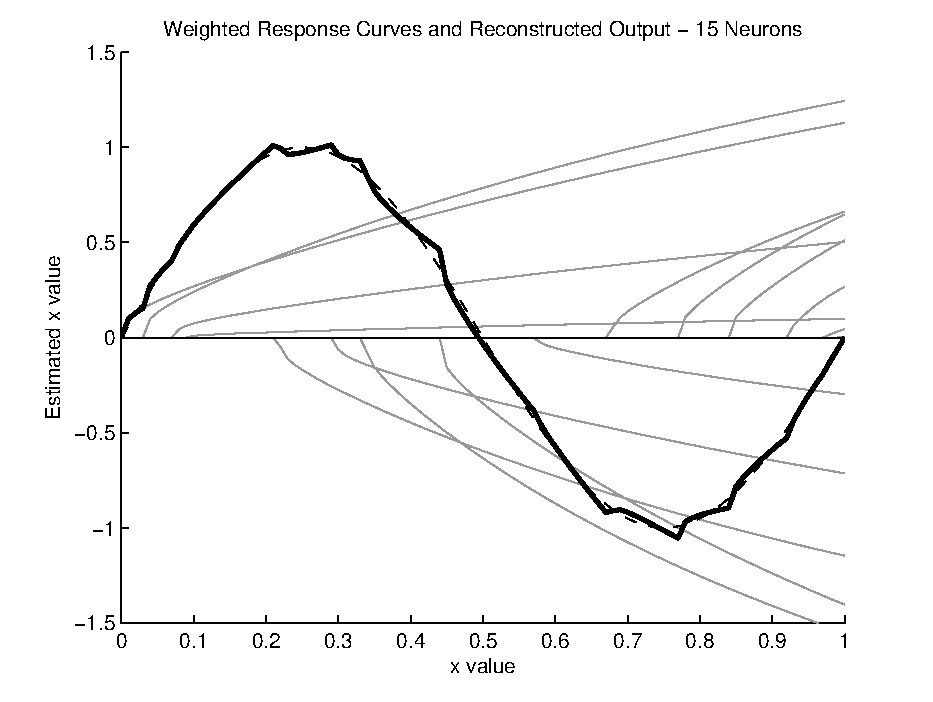
\includegraphics[width=0.45\columnwidth]{lif_func_out_15}
%   \caption{Illustration showing how the tuning curves of a population of LIF
%     neurons can be linearly combined to estimate a nonlinear function, in this
%     case $\sin(2\pi x)$. From \cite{Choo2010}.}
%   \label{fig:dec-func}
% \end{figure}

Note that this method
of computing nonlinear transformations
requires that all of the vectors
participating in the transformation
must be represented by a single ensemble.
Therefore, in order to compute
a function $f(\V{x_1}, \V{x_2})$,
a new ensemble must be created
that will represent
a vector in a space that is the concatenation
of the spaces in which $\V{x_1}$
and $\V{x_2}$ reside.

\subsection{Dynamics}

Dynamical systems have been used effectively
for control problems in several domains.
As animals are successful controllers
of cognitive and motor actions,
implementing dynamical systems
with spiking neurons seems a natural fit.
In the NEF, dynamics are implemented
by interpreting the vector
represented by some ensemble as
the state of a dynamical system,
which can implement differential equations
through recurrent connections.
No additional techniques are required
to compute recurrent connections;
the transformation principle
is used as previously described.
The dynamics principle
is instead a type of network architecture
(see Figure~\ref{fig:dynamics}) that can
implement differential equations
as are descried in dynamical systems
and control theory.

\fig{dynamics}{0.6}{???}{???}
% ??? fig 6.5 from dewolf, or htbab 2.12

The architecture depicted in Figure~\ref{fig:dynamics}
implements a linear control system,
and can be expressed as
\begin{equation}
  \V{\dot{x}}(t) = \V{Ax}(t) + \V{Bu}(t),
\end{equation}
where $\V{A}$ is the dynamics matrix
and $\V{B}$ is the input matrix.
Normally, transforming this equation
into Laplace space results
results in dynamics scaled by
the filter $H(s) = \frac{1}{s}$.
However, the actual dynamics of the system
are based on the synaptic dynamics,
$h(t)$ from equation~\eqref{...}.
The Laplace transform of $h(t)$ is
$H'(s) = \frac{1}{1 + s\tau}$.
By accounting for the difference
between these two filters
(see \cite{eliasmith2004,eliasmith2013}
for a full derivation),
we get
\begin{align}
  \V{A'} &= \tau \V{A} + \V{I} \\
  \V{B'} &= \tau \V{B},
\end{align}
where $\V{I}$ is the identity matrix.

Equations~\eqref{...} and \eqref{...}
allow us to implement any linear dynamical system
in spiking neural networks
by setting up the recurrent connection
from the ensemble representing the system state
to compute the linear transform $\tau \V{A} + \V{I}$,
and setting the transform on the connection
from the input ensemble
to the system state ensemble
to have weight $\tau \V{B}$.

Nonlinear dynamical systems can also be implemented
with a similar approach;
in essence, all that is required is to
recognize that the synaptic filter $h(t)$
introduces an exponential ``forgetting''
of the system state
which must be accounted for by scaling
connections with the time constant $\tau$.

\section{Semantic Pointer Architecture (SPA)}
\label{sec:methods-spa}

The Neural Engineering Framework (NEF)
allows us to manipulate dynamical systems
in $n$-dimensional vector spaces
with spiking neurons,
which is essential for
the continuous temporal tasks
involved in speech.
However, speech also connects
to linguistic and cognitive systems
that have traditionally been described
with static symbols
and rule-based algorithms.
The Semantic Pointer Architecture (SPA; \cite{eliasmith2013})
provides a method to implement
symbol-like representations
and transformations in spiking neural networks,
building on the NEF.

The crux of the SPA is to implement
the operations in
a vector symbolic architecture
using the NEF.
While many vector symbolic architectures exist,
the SPA specifically uses
Holographic Reduced Representations (HER),
developed by \cite{plate1994},
as it scales well to high dimensional spaces,
and can be implemented naturally
with the NEF.

\subsection{Representation}

As in all vector symbolic architectures,
we associate a real-valued vector
with every ``symbol''
in the vocabulary associated with
the problem domain.
In the case of speech,
the vocabulary depends on
the specific subproblem,
but could be composed
of phoneme symbols,
syllable symbols,
word symbols, and so on.

In order to robustly implement
the transformations discussed
in the subsequent section,
we use vectors of unit length
when possible.
When we have no information
about the structure of a particular pointer,
we randomly generate it
by sampling from a normal distribution
for each dimension of the vector,
then normalizing by the L2-norm
of the vector.


When we do have information about
the structure of vector,
we construct them by
using the transformations below
with randomly generated vectors,
or vectors learned through
unsupervised methods.
However, it is possible that
the transformations below
result in vectors that are
no longer of unit length.
To limit the number of situations
in which this occurs,
we can use random \textit{unitary} vectors
\cite{plate1994}.

A unitary vector is a vector with
the same exact inverse
as its approximate inverse.
The exact inverse of a vector
is sensitive to noise,
which is prevalent in biological systems.
Therefore, when a transformation needs to
invert a vector,
it instead uses an approximation
of the inverse called the \textit{involution}.
Given a vector $\V{A}$, the involution
of that vector $\V{A'}$,
is a rearrangement of the vector dimensions;
specifically,
\begin{equation}
  \V{A'} = A'_{i} = A_{-i \bmod n},
\end{equation}
where $n$ is the number of dimensions,
and $\bmod$ is the modulo operator.
For example, if $\V{A} = [a_0, a_1, a_2, a_3]$,
then $\V{A'} = [a_0, a_3, a_2, a_1]$.
It is apparent that $\V{A''} = \V{A}$,
hence its usefulness as an approximate inverse.

The approximate inverse is equal to the
inverse when the components
of the discrete Fourier transform
of the vector have unit magnitude.
Therefore, to generate a random unitary vector,
we generate a random unit vector,
and then normalize
the frequency components;
specifically,
\begin{equation} \label{unitary}
  \V{A}^1 = \text{IDFT}\left(
    \frac{\text{DFT}(\V{A})}{\Vert\text{DFT}(\V{A})\Vert}\right),
\end{equation}
where $\Vert\cdot\Vert$ is the L2-norm.
Note that the a unitary vector generated
with equation~\eqref{unitary}
is still a unit vector.

\subsection{Transformation}
\label{sec:spa-transformation}

Vector symbolic architectures
define two transformations
that are necessary
to implement rule-like behavior:
merging and binding.
Merging takes two vectors
and combines them such that
the resulting vector
is similar to both of the input vectors.
Binding takes two vectors
and combines them such that
the resulting vector
is dissimilar from either of the input vectors,
but the input vectors can be recovered
through an unbinding process.

In HRRs,
the merging transformation,
which we will denote with $\oplus$,
is vector superposition.
\begin{equation}
  \V{A} \oplus \V{B} = [A_0 + B_0, A_1 + B_1, ...]
\end{equation}
Since the new representation
is a linear combination of
the two vectors,
it is similar to both,
as long as the two vectors
are not too dissimilar.
Note that similarity in SPA can
be computed either by
the dot product between two vectors,
\begin{equation}
  \V{A} \cdot \V{B} = \sum_{i=0}^{n-1} A_i B_i,
\end{equation}
or the cosine similarity,
which is the dot product normalized
by the length of the two vectors; i.e.,
\begin{equation}
  \cos(\theta) = \frac{\V{A} \cdot \V{B}}{\Vert\V{A}\Vert \Vert\V{B}\Vert}
    = \frac{\sum_{i=0}^{n-1} A_i B_i}
           {\sqrt{\sum_{i=0}^{n-1} A_i^2} \sqrt{\sum_{i=0}^{n-1} B_i^2}}.
\end{equation}

The binding transformation in HRRs,
which we will denote with $\bind$,
is circular convolution.
While circular convolution
is defined as
\begin{equation}
  \V{A} \bind \V{B} = \sum_{i=0}^{n-1} A_{i \bmod n}B_{j-i \bmod n},
    \text{ for } j=0, \ldots, n-1,
\end{equation}
we can reduce the computational complexity
of the transform
by computing it as the
product of discrete Fourier coefficients.
Specifically,
\begin{equation}
  \V{A} \bind \V{B} = \text{IDFT}\left[
    \text{DFT}(\V{A}) \circ \text{DFT}(\V{B})\right],
\end{equation}
where $\circ$ is the Hadamard (element-wise) product.
In addition to lowering
the computational complexity,
the DFT and IDFT functions are linear,
making them easy to implement
in a spiking neural network.
Also, observe that in this formulation,
convolving with a unitary vector,
which has DFT coefficients of unit magnitude,
does not change the magnitude
of the resulting element-wise product.
Therefore, when convolving a unit vector
with a unitary vector,
we obtain another unit vector,
which is a useful property
in many situations.

In order to recover inputs,
we can ``unbind'' the bound vector
to retrieve one input vector
by binding with the approximate inverse (involution)
of the other input vector.
\begin{equation}
  (\V{A} \bind \V{B}) \bind \V{A'} \approx \V{B}
\end{equation}
Note that unbinding is approximate;
since the binding operation
mixes the two vectors together,
they cannot be recovered exactly.
However, vectors can be subsequently
``cleaned up'' to known
vocabulary items using an autoassociative memory.

It is important to note that
the HRR definitions for merging and binding
do not change the dimensionality
of the vector space, unlike other VSAs
(e.g., \cite{smolensky1990}).
One can therefore think of the
merging and binding operators
as compressing the information
in the input vectors.
The Semantic Pointer Architecture
gets its name from the idea that
the vectors used
in any reasonably large SPA network
are made up of compressed versions
of other vectors in vocabularies
distributed among many interacting networks.
The vectors in these vocabularies
have meaning.
Since the compressed representations
can be decompressed through unbinding,
we say that they ``point''
to deeper semantics,
analogous to how a pointer in computer science
points to an area of memory.
Semantic pointers, however,
also contain shallow semantics,
so that the compressed
representations themselves
can be used to implement cognitive behaviors.
From here on, We will refer to
the vectors in a conceptual vocabulary
as semantic pointers.

The SPA has been used to implement
models of large-scale knowledge representation
using WordNet \cite{crawford2015},
serial working memory \cite{choo2010},
and other cognitive tasks.
An integrated model called Spaun
combined several previous models
in a single unified model
that performed eight cognitive tasks
with no reorganization.
In these tasks, input was provided
through a simulated visual system,
and output was produced
as motor commands driving
a three link arm model
\cite{eliasmith2012,eliasmith2013}.

\section{Nengo software}
\label{sec:nengo}

Nengo is a piece of software
for designing and simulating
models using the representations,
transformations, and dynamics
of the NEF and SPA
\cite{bekolay2013}.
The NEF provides a level of abstraction
that allows modelers to generate
spiking neural networks
that implement dynamic transformations
in vector spaces.
The SPA provides a level of abstraction
on top of that
to allow modelers to generate
NEF networks to perform
cognitively relevant operations
on symbol-like representations.
Nengo provides modelers
a level of abstraction to
define and simulate NEF and SPA models
using the Python programming language.

Nengo defines a set of six objects
used to construct a spiking neural model.
The \textit{Ensemble} is
a population of spiking neurons
that represents a vector over time.
It presents a simplified interface
allowing modelers to specify
details important for modeling,
rather than manually specifying
all model parameters;
for example, instead of specifying
the gain and bias
(see Equation~\eqref{eq:encoding}),
one can specify the desired
$x$-intercepts and maximum firing rates
of the ensemble's tuning curves.
Additionally, one can specify
these parameters in terms of
probability distributions
to be sampled,
rather than specifying a value for each neuron.

\textit{Nodes} provide output
to the model, or gather input from the model,
but does so without using spiking neurons.
Nodes allow models to interact with environments.
Connecting from a node provides input
to the model, which could be
a direct current injection,
a list of vectors to be encoded,
or data coming from a sensor
like a spiking camera.
Connecting to a node allows it
to do arbitrary processing on
model outputs;
nodes can record model outputs,
update plots in real time,
or drive a physical robot arm.

\textit{Connections} encapsulate
the flow of information between two objects.
For connections between ensembles,
connections can be specified in vector space
as a function of the input ensemble,
or in neuron space
by fulling specifying the connection weight matrix.
When functions are provided,
the decoder solving process
(see Equation~\eqref{eq:decoding})
is done automatically,
though parameters affecting
how the decoders are solved for
can be specified.

\textit{Probes} specify quantities
in the model that should be recorded
for analysis and visualization.
Nengo by itself does not
impose any constraints on how
that data is used;
for the models in this thesis,
the data was analyzed with
NumPy \cite{vanderwalt2011}
and SciPy \cite{jones2014}
and visualized with
Matplotlib \cite{hunter2007}
and Seaborn \cite{waskom2014}.
However, other analysis and plotting packages
could be used.

\textit{Networks} are a collection of
the other five objects
(and possibly other networks),
and provide the primary abstraction
for defining large models
in few lines of Python code.
The SPA transformations
described in the previous section
are implemented as a several
interacting networks.
The models described
in Chapter~\ref{chapt:implementation} consist
of some instances of
these SPA networks,
and several networks
that we have constructed.

Python scripts using Nengo to construct
the models discussed in the next chapter
are available at \url{https://github.com/tbekolay/phd},
and in simplified form in the appendix.

\subsection{Integrating Brian in Nengo}

As discussed in Section~\ref{sec:brian-hears},
we use the Brain neural simulator's
Brian Hears package
to simulate auditory periphery models.
As our models are implemented in Nengo,
it is necessary for Brian and Nengo
to interact in some way.
The naive approach,
which is necessary in many simulation environments,
is to manually step through both simulators,
copying the data produced by Brian
to Nengo when the Nengo simulator advances.
A faster approach would be to
pre-generate all of the data
produced by Brian
and feed that in as
static input.
However,
then the Brian simulation could not
use input from the Nengo simulator;
a bidirectional interface
is important for future closed loop models.

The integration is instead done
through a Nengo node.
The function attached to the node
contains the state of the Brain simulation,
which can be advanced at a different rate
as the Nengo simulation if desired.
In addition to collecting
data from the auditory filters,
the node can update the
sound associated with
the auditory filter,
allowing for a bidirectional interface.
Updating the sound would normally
clear the state of the auditory filter,
so we instead subclass Brain's
\textit{Sound} object
and provide samples from
Nengo when needed.
